\documentclass{report}
\usepackage{graphicx} % Required for inserting images
\usepackage[italian]{babel}
\usepackage{tikz}
\usepackage{hyperref}
\usepackage{amsmath}
\usepackage{xcolor}
\usepackage{float}
\usepackage{soul}
\usepackage{listings} % Per evidenziare il codice

\definecolor{lightgray}{rgb}{0.9,0.9,0.9} % Definizione colore sfondo
\definecolor{darkgreen}{rgb}{0.0, 0.5, 0.0}

\lstset{
    backgroundcolor=\color{lightgray}, % Sfondo grigio
    basicstyle=\ttfamily, % Font monospaziato
    % frame=single, % Bordo attorno al codice
    tabsize=4, % Dimensione tabulazione
    breaklines=true, % Permette di andare a capo automaticamente
    numbers = left,
    numberstyle=\small\color{gray}
}

\title{\huge\textbf{{Intelligent System for Industry, Supply Chain and Environment}}}
\date{Parte I}

\begin{document}

\maketitle

\tableofcontents
\newpage

\chapter{Introduzione}

\section{What is an intelligent system (IS)}
\begin{center}
    \textit{a computer-based system that aims to replicate human cognitive abilities such as learning, perception, reasoning, and decision-making. }
\end{center}

\noindent By utilizing Machine Learning (ML), and other related technologies, these systems are capable of processing and analyzing data to perform tasks that typically require human intelligence, make predictions, or provide insights

\chapter{Legislation, Artificial and human learning, Gestalt, applications and opinions about AI}
\section{Laws about AI in Europe}
\noindent The AI Act is a European law on artificial intelligence (AI), the first comprehensive law on AI by a major regulator anywhere. 
The AIA was published in the Official Journal of the EU on 12 July 2024 and entered into force on 1 August 2024 . 


\noindent \textbf{\textit{Why do we nee rules on AI?}}
\begin{itemize}
    \item To avoid undesirable outcomes
    \item It is often not possible to find out why an AI system has made a decision or prediction and taken a particular action. 
    \item It may become difficult to assess whether someone has been unfairly disadvantaged, such as in a hiring decision or in an application for a public benefit scheme
\end{itemize}

According to the European Union's Artificial Intelligence Act (AI Act), an AI system is defined as: 
\begin{center}
    \textit{"a machine-based system designed to operate with varying levels of autonomy and that may exhibit, for explicit or implicit objectives , infers from the input it receives how to generate outputs such as predictions , content , recommendations, or decisionsthat can influence physical or virtual environments"}
\end{center}


\subsection{Four risk levels}
\begin{figure}[H]
    \centering
    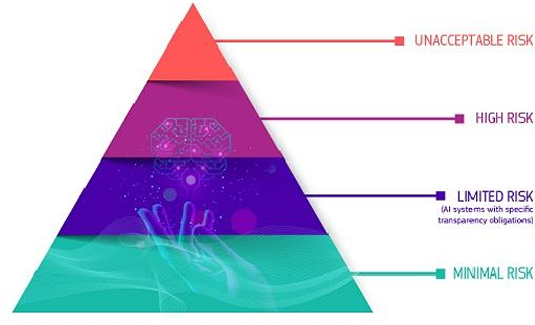
\includegraphics[width=0.6\linewidth]{images/piramide.png}
\end{figure}

\begin{itemize}
    \item \textbf{Unacceptable risk:} All AI systems considered a clear threat to the safety, livelihoods and rights of people will be banned
    \item \textbf{High risk:} \begin{itemize}
        \item critical infrastructures (e.g. transport), that could put the life and health of citizens at risk;
        \item educational or vocational training, that may determine the access to education and professional course of someone’s life (e.g. scoring of exams);
        \item safety components of products (e.g. AI application in robotassisted surgery);
        \item employment, management of workers and access to selfemployment (e.g. CV-sorting software for recruitment procedures);
        \item essential private and public services (e.g. credit scoring denying citizens opportunity to obtain a loan);
        \item law enforcement that may interfere with people’s fundamental rights (e.g. evaluation of the reliability of evidence);
        \item migration, asylum and border control management (e.g. verification of authenticity of travel documents);
    \end{itemize}
    \item \textbf{Limited risk:} refers to AI systems with specific transparency obligations
\end{itemize}

\end{document}